\chapter{Tổng quan nghiên cứu}
\label{chap:1tqnc}
\section{Giới thiệu robot tự hành}

% - Thế nào là robot tự hành thông minh
% - ứng dụng của robot tự hành thông

%%% Tài liệu tham khảo:
% http://ais.informatik.uni-freiburg.de/teaching/ss18/robotics/ Bài Introduction
% 

Trước đây, nghành robotics tập trung vào nghiên cứu và chế tạo cánh tay robot công nghiệp. Nó được coi như là robot truyền thống (\figurename{\ref{fig:RBCongNghiep}}). Bởi vậy khi nói đến thuật ngữ robot người ta thường nghĩ ngay đến cánh tay robot công nghiệp. \figurename{\ref{fig:RBCongNghiep}} là hình ảnh các cánh tay robot đang làm việc trong khâu sơn khung xe oto. Chúng ta không thấy bóng dáng con người ở trong bức hình này, bởi vì robot công nghiệp truyền thống phải làm việc trong không gian cách ly với con người, có hàng rào bảo vệ vì các lý do an toàn, con người không thể làm việc cùng không gian với robot. 

\begin{figure}[hpt]
  \centering
  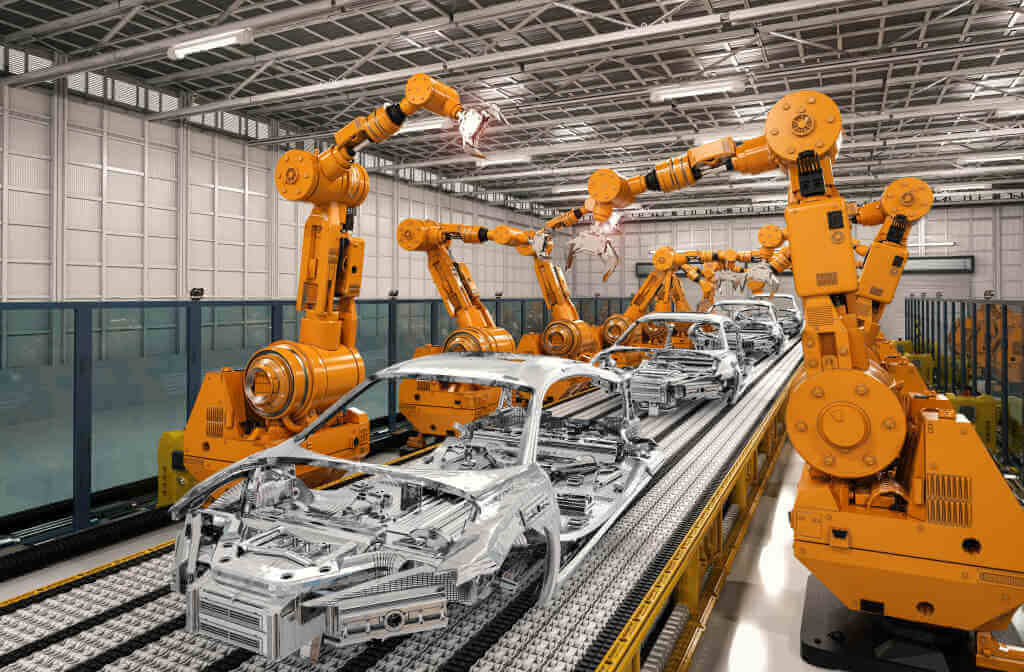
\includegraphics[width=10cm]{figures/IndustrialRobot.jpg}
  \caption{Robot công nghiệp [Nguồn: Internet]}
  \label{fig:RBCongNghiep}
\end{figure}

Bên cạnh đó, robot di động (mobile robot) truyền thống thực hiện các nhiệm vụ di chuyển trên quỹ đạo xác định trước. Robot di động cũng hoạt động dựa trên các khối chương trình được lập trình sẵn. Các phương pháp điều khiển như điều khiển bằng tay thông qua bảng điều khiển, qua sóng RF, wifi... hay di chuyển bám đường chỉ dẫn gắn ở dưới sàn, đọc mã QR, bar. Robot dạng này bị hạn chế về không gian hoạt động. Việc thiết lập, cấu hình nhà máy, không gian làm việc cho robot hoạt động hết sức tốn kém về chi phí và thời gian mà lại kém linh hoạt.

Ngày nay, robot có xu hướng đi ra khỏi không gian nhà máy, xuất hiện nhiều loại robot như: robot giải trí (\figurename{\ref{fig:rbMoi-a}}), robot dịch vụ cá nhân (\figurename{\ref{fig:rbMoi-b}}) (như máy tính cá nhân), robot trong y tế (\figurename{\ref{fig:rbMoi-c}}); các loại robot tự động trong công nghiệp như robot hái quả (\figurename{\ref{fig:rbMoi-d}}), phun thuốc trong nông nghiệp, robot thông minh tác hợp trong công nghiệp; robot đi tới các môi trường mà con người không tới được như trong lòng đất dưới nước, trên không, trong vũ trụ...
\begin{figure}
	\centering
	\subfloat[][]{
          \label{fig:rbMoi-a}
          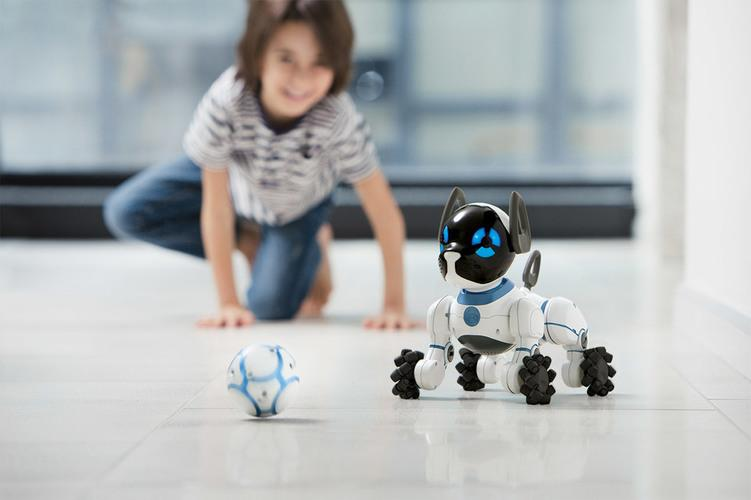
\includegraphics[height=5cm]{figures/c1_entertainmentRobot.jpg}}
        \subfloat[][]{
          \label{fig:rbMoi-b}
          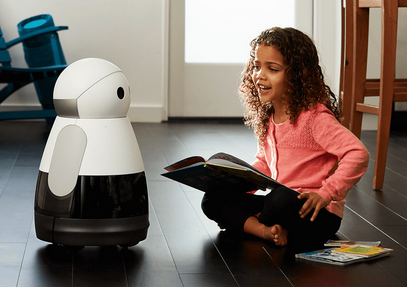
\includegraphics[height=5cm]{figures/c1_personalServiceRobot.png}}
        \hspace{8pt}
        \subfloat[][]{
          \label{fig:rbMoi-c}
          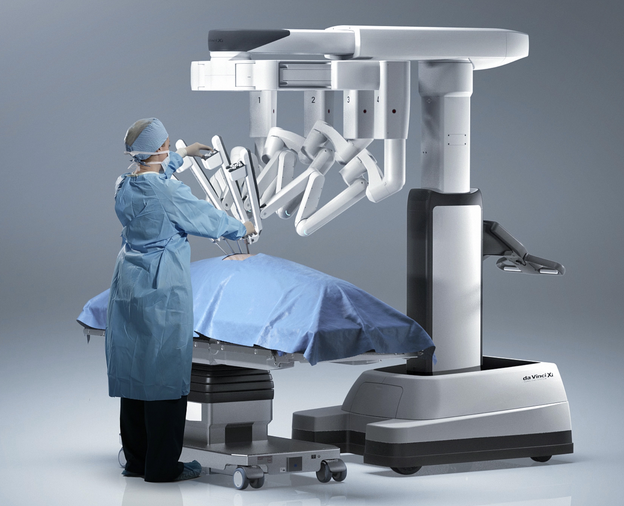
\includegraphics[height=4.6cm]{figures/c1_medicalRobot.png}}
        \subfloat[][]{
          \label{fig:rbMoi-d}
          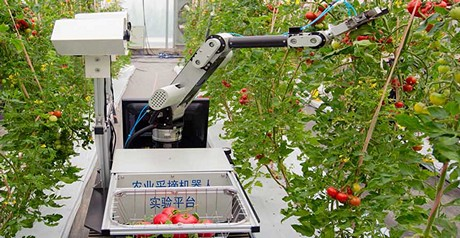
\includegraphics[height=4.6cm]{figures/c1_harvestingRobot.jpg}}
	\hspace{8pt}
	\caption[]{Một số loại robot mới}
	\label{fig:rbMoi}
\end{figure}

\begin{figure}[htp]
  \centering
  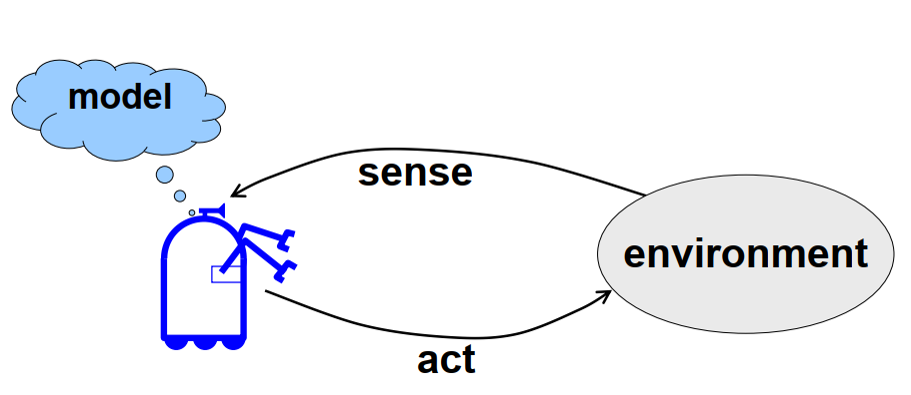
\includegraphics[width=12cm]{figures/c1_AutonomousRBModel.png}
  \caption{Mô hình hệ thống robot tự hành}
  \label{fig:MohinhRB}
\end{figure}

%Trong đó, hệ thống robot tự hành là một dạng robot điển hình cho thế hệ robot mới ngày nay và đang phát triển rất mạnh mẽ. Hệ thống robot tự hành là hệ thống hoạt động như mô hình \figurename{\ref{fig:MohinhRB}}: Robot cảm nhận môi trường thông qua hệ thống cảm biến. Mô hình hóa môi trường sau đó thực hiện các hành động phản ứng lại với môi trường. Các hoạt động cảm nhận môi trường như đo khoảng cách bằng cảm biến siêu âm, hồng ngoại, lidar hay ứng dụng deep learning để nhận dạng đồ vật, người... Các hành động phản ứng có thể là xây dựng bản đồ, thực hiện di chuyển, thực hiện tránh vật, gắp vật...

Robot tự hành thông minh là loại robot di động, có thể cảm nhận, mô hình hóa môi trường xung quanh nó. Thực hiện các hành động di chuyển mà không cần sự giám sát cũng như điều khiển trực tiếp từ con người (\figurename{\ref{fig:MohinhRB}}).

% Có nên thêm phần giới thiệu các robot dựa trên robot tự hành:

\section{Ứng dụng của robot tự hành thông minh}
\label{sec:ungdung}

Với sự thông minh và cực kì linh hoạt của nó, robot tự hành thông minh có rất nhiều ứng dụng. Về cơ bản, nó là nền tảng di chuyển cho tất cả các loại robot di động thông minh ngày nay. Một số sản phẩm ứng dụng trong nhà như:

\begin{itemize}
\item Các ứng dụng trong nhà như robot hút bụi thông minh, robot dịch vụ, robot vận chuyển trong các kho hàng\dots
\item Các ứng dụng ngoài trời như robot cắt cỏ, chăm sóc cây trồng...
\item Ở các không gian mà con người không tới được như robot thám hiểm dưới nước, trong lòng đất, trên không trung trên các hành tinh khác...
\item Tại các khu vực nguy hiểm như khu vực nhiễm chất phóng xạ, chữa cháy...
\item Và đặc biệt, robot giao hàng tự động, xe tự lái đang phát triển rất nhanh trong những năm gần đây 
\end{itemize}

\section{Các bài toán trên robot tự hành thông minh}

% - Nêu qua concept về điều khiển robot, tạo bản đồ, định vị, path planning, điều hướng, tránh vật cản
Một số bài toán chính trong robot tự hành như sau (\cite{Wise}):

\textbf{Cảm biến:} Robot tự hành thông minh cần một số loại cảm biến để có thể hiểu được môi trường, định vị và di chuyển tránh vật cản. 

Có rất nhiều loại cảm biến, để cảm nhận được đa dạng thông tin của môi trường. Có thể chia làm các nhóm như sau:
\begin{itemize}
\item Khoảng cách 1D: Cảm biến khoảng cách hồng ngoại, siêu âm
\item Khoảng cách 2D: Lidar
\item Cảm biến 3D: Có nhiều loại cảm biến 3D như Intel realsense, Microsoft Kinect, Asus Xction...
\item Ước tính trạng thái robot: GPS, IMU
\item Cảm biến lực, momen, cảm biến chạm...
\item Âm thanh, giọng nói như microphone, microphone array
\item Các loại camera 2D
\end{itemize}

\textbf{Odometry}: là bài toán sử dụng thông tin nhận được từ các cảm biến nhận biết sự di chuyển của robot để ước tính sự thay đổi vị trí của robot qua thời gian. Odometry được sử dụng trong hầu hết các robot tự hành.

\textbf{Định vị}: Bài toán định vị giúp trả lời câu hỏi robot đang ở đâu, từ đó có cơ sở để thực hiện các tác vụ khác như tạo bản đồ, xác định hướng di chuyển.

\textbf{Xây dựng bản đồ}: Dự trên dữ liệu từ các loại cảm biến, từ odometry và định vị robot, robot sử dụng các thuật toán để xây dựng bản đồ của môi trường.

\textbf{Điều hướng robot}: Từ bài toán định vị và khi có được bản đồ và nhiệm vụ di chuyển từ vị trí hiện tại tới một vị trí đích. Robot sẽ tính toán qũy đạo và điều khiển di chuyển tới đích.

\textbf{Tránh vật cản}: Trong quá trình di chuyển, robot phải phát hiện được các vật cản (bao gồm cả tĩnh và động) và tránh vật cản, sau đó thiết lập lại quỹ đạo di chuyển tới đích.

Vấn đề xuyên suốt trong các bài toán của robot tự hành thông minh đó là các dữ liệu đều không chắc chắn, các bài toán trên đều dựa vào các mô hình xác suất để mô hình hóa được trình bày trong tài liệu \cite{Sebastian2005}.

% Thêm một đoạn dẫn liên kết vào đây

\section{Các nghiên cứu tránh vật cản trong robot tự hành thông minh}
\label{sec:tranhVatCan_ref}

% Review các bài báo về tránh vật cản trong robot tự hành
% Chỉ ra các ưu, nhược điểm của các phương pháp như được nêu trong các bài báo trên
Khả năng phát hiện và tránh vật cản theo thời gian thực là rất quan trọng trong robot tự hành. Do đó có rất nhiều nghiên cứu về giải pháp cho vấn đề này. Có nhiều loại cảm biến được sử dụng, nhiều giải thuật được sử dụng. Các loại cảm biến sử dụng như cảm biến khoảng cách hồng ngoại, siêu âm với ứng dụng trên các thiết bị nhúng cấu hình thấp \cite{dongyue2013, Susnea2009}. Các phương pháp sử dụng cảm biến laser radar được trình bày trong \cite{Gao2019, Wu2015, Peng2015}. Các thuật toán phổ biến được dùng để phát hiện và tránh vật cản như Virtual Force Field (VFF) \cite{Borenstein1989}, Vector Field Histogram (VFH) \cite{Borenstein1991}, Dynamic Window Approach (DWA) \cite{Fox1997}\ldots

\subsection{Thuật toán Virtual Force Field (VFF)}

Được áp dụng cho điều khiển tránh vật cản trình bày trong \cite{Borenstein1988,Borenstein1989}. Ý tưởng của giải thuật này là tạo một ô lưới quanh robot. Khi có dữ liệu có vật cản từ cảm biến, ô tương ứng sẽ được đặt là bị chiếm dụng bởi vật cản với một tỉ số chiếm dụng (thể hiện cho sự không chắc chắn), nhiệm vụ của thuật toán là tính toán một lực để đưa robot xa khỏi ô bị chiếm dụng đó.


\begin{equation}
  F(i,j) = \frac{{F}_{cr}C(i,j)}{{d}^{2}(i,j)}\left [\frac{{x}_{t}-{x}_{0}}{d(i,j)}\dot{x} + \frac{{y}_{t}-{y}_{0}}{d(i,j)}\dot{y} 
  \right ]
\end{equation}
Trong đó: 

\begin{tabular}{ll}
  $F(i,j)$      & Lực ảo chống lại vật cản tại ô (i,j) \\
  ${F}_{cr}$    & Hằng số lực chống lại vật cản  \\
  $d(i,j)$      & Khoảng cách giữa ô (i,j) và robot \\
  ${C}_{i,j}$   & Độ chắc chắn tại ô (i,j)  \\
  ${x}_{0}, {y}_{0}$ & Tọa độ robot \\
  ${x}_{i}, {y}_{j}$ & Tọa độ của ô (i,j)
\end{tabular}

Lực ${F}_{r}$ đưa robot tránh khỏi các vật cản xuất hiện xung quanh robot là tổng của các lực tại mỗi ô lưới. 

\begin{equation}
  {F}_{r} = \sum\limits_{i,j}{F(i,j)}
\end{equation}

Trong khi đó, lực ${F}_{t}$ kéo robot đi từ điểm hiện tại tới điểm đích như sau: 

\begin{equation}
  {F}_{t} = {F}_{ct} \left [\frac{{x}_{t}-{x}_{0}}{d(t)}\dot{x} + \frac{{y}_{t}-{y}_{0}}{d(t)}\dot{y} 
  \right ]
\end{equation}

Trong đó: 

\begin{tabular} {ll}
  ${F}_{ct}$    & Hằng số lực kéo robot tới đích \\
  $d(t)$        & Khoảng cách giữa robot và điểm đích \\
  ${x}_{t}, {y}_{t}$ & Tọa độ của điểm đích
\end{tabular}

\begin{figure}[htp]
  \centering
  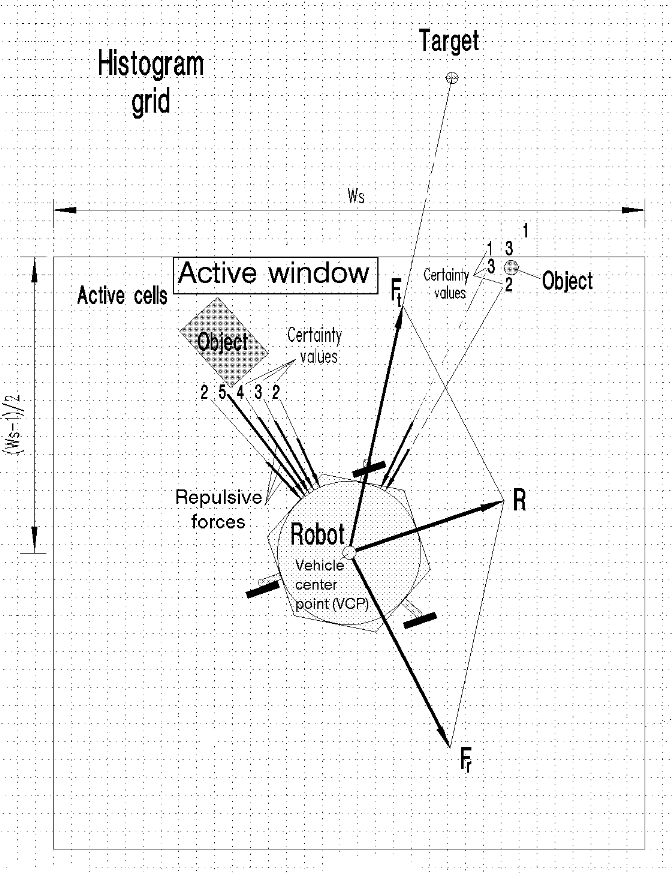
\includegraphics[width=0.5\linewidth]{figures/VFFconcept.png}
  \caption{Virtual Force Field \cite{Koren1991}}
  \label{fig:VFFconcept}
\end{figure}

Hợp lực của 2 loại lực này là lực chính kéo robot di chuyển.

\begin{equation}
  R = {F}_{t} + {F}_{r}
\end{equation}


Từ đó tính được hướng di chuyển của robot để điều khiển bánh xe di chuyển, đưa robot tới đích và tránh được vật cản. Theo \cite{Borenstein1988}, phương pháp này có một số ưu điểm như sau:
\begin{itemize}
  \item Phương pháp này không xác định được đường viền cạnh của vật cản, nhưng có thể xác định được cụm các vị trí có vật cản.
  \item Phương pháp này không yêu cầu robot phải dừng lại để thực hiện lấy dữ liệu và tính toán. Trong điều kiện lý tưởng, phương pháp này giúp robot có thể tránh được tất cả vật cản trong khi vẫn di chuyển với vận tốc tối đa.
  \item Việc cập nhật bản đồ lưới và điều hướng sử dụng bản đồ lưới là hai nhiệm vụ hoàn toàn không phụ thuộc vào nhau, nhưng có thể đồng bộ với nhau để tối ưu tính toán. 
  \item Phương pháp này có thể dễ dàng tích hợp nhiều loại cảm biến để bổ sung thông tin vào bản đồ ô lưới. 
\end{itemize}

Tuy nhiên, theo \cite{Koren1991}, phương pháp này có một số điểm hạn chế như: Các trường hợp mắc bẫy do cực tiểu địa phương, không thể di chuyển qua giữa các vật cản gần nhau, lưỡng lự khi có vật cản, lưỡng lự trong lối đi hẹp

Do đó, phương pháp Vector Field Histogram cải thiện các hạn chế của phương pháp Vector Force Field

\subsection{The Vector Field Histogram}
\label{sub:VFH}
Phương pháp VFH \cite{Borenstein1991} sử dụng kĩ thuật hai giai đoạn giảm dữ liệu và ba mức thể hiện dữ liệu:

\begin{itemize}
  \item Mức biểu diễn dữ liệu cao nhất giữ mô tả chi tiết của môi trường robot, bản đồ lưới 2 chiều được cập nhật liên tục theo thời gian thực như trong phương pháp VFF. 
  \item Mức ở giữa, một biểu đồ H một chiều được dựng quanh vị trí tức thời của robot. H bao gồm $n$ góc với độ rộng $\alpha$, phép chuyển đổi từ C sang H. 
  \item Mức biểu diễn dữ liệu thấp nhất là đầu ra của thuật toán VFH: các giá trị tham chiếu cho động cơ và bánh xe điều khiển robot. 
\end{itemize}

% \begin{figure}[htp]
%   \centering
%   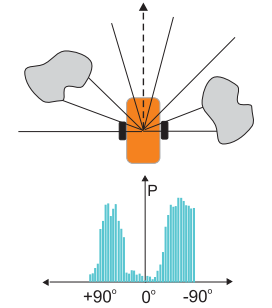
\includegraphics[]{figures/VFH.png}
%   \caption{Virtual Force Field \cite{Susnea2009}}
%   \label{}
% \end{figure}

\begin{wrapfigure}{r}{0.4\textwidth}
  \centering
  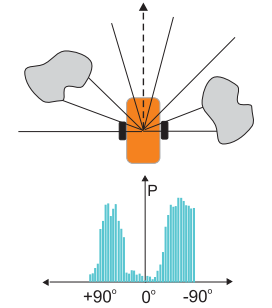
\includegraphics[width=0.4\textwidth]{figures/VFH.png}
  \caption{Vector Field Histogram \cite{Susnea2009}}
  \label{fig:VFH}
\end{wrapfigure}

Phương pháp này có thể phát hiện được lối đi đủ cho robot đi qua giữa các vật cản.  Phương pháp VFF dễ bị ảnh hưởng bởi sai số của cảm biến, với phương pháp này, sử dụng làm mịn biểu đồ H đã giảm trọng số của các giá trị sai ngẫu nhiên của cảm biến, do đó phương pháp này mạnh hơn phương pháp VFF. Vẫn bị hiện tượng mắc bẫy khi vào các trường hợp "dead-end" (đường cụt) do sử dụng phương pháp cục bộ. Tốc độ di chuyển tối đa khi điều khiển robot bằng VFH bị giới hạn bởi tốc độ lấy mẫu của cảm biến. 

Dựa trên phương pháp này, \cite{Ulrich1998} đã đề xuất phương pháp được gọi là VFH+ thực hiện 4 giai đoạn giảm dữ liệu từ bản đồ lưới chiếm dụng hai chiều xuống thành dữ liệu điều khiển hướng di chuyển của robot. Sử dụng một số cải tiến để giúp robot có thể di chuyển tốt hơn.
  
\subsection{Phương pháp "Bong bóng phản ứng" tránh vật cản}

\begin{wrapfigure}{r}{0.5\textwidth}
  \centering
  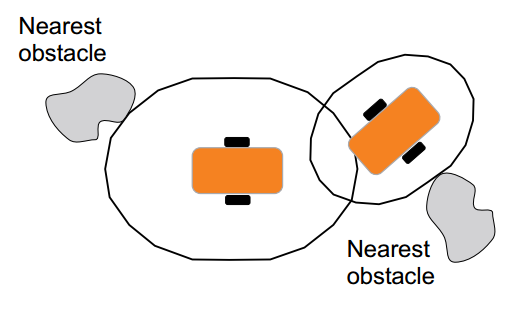
\includegraphics[width=0.5\textwidth]{figures/bubble-band.png}
  \caption{Bong bóng phản ứng \cite{Susnea2009}}
  \label{fig:bubble-band}
\end{wrapfigure}

Phương pháp này được đề xuất trong \cite{Quinlan1993}, phương pháp này định nghĩa một "bong bóng" bao quanh robot thể hiện không gian lớn nhất có thể di chuyển mà không gặp vật cản. Hình dạng và kích thước của bong bóng được xác định đơn giản dựa trên hình dạng vật lý của đế robot và từ thông tin của cảm biến (như \figurename{\ref{fig:bubble-band}}).

\begin{figure}
	\centering
	\subfloat[][]{
          \label{fig:bb-computeAngle}
          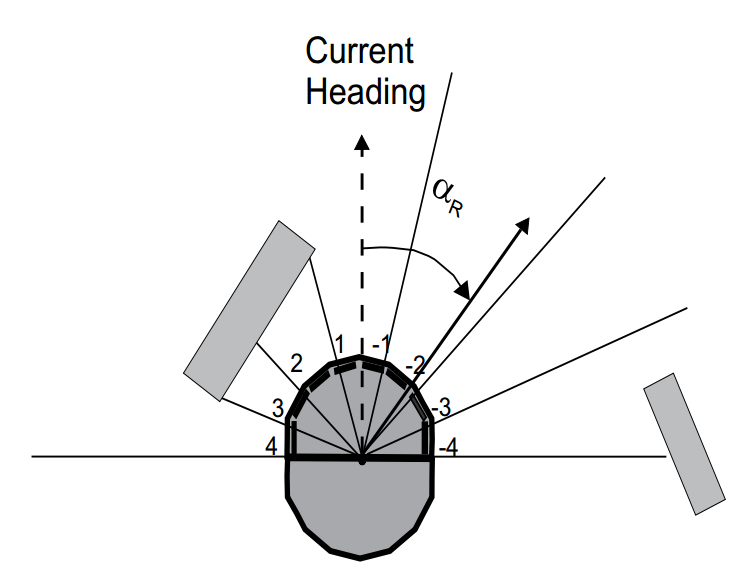
\includegraphics[width=0.45\textwidth]{figures/computeReboundAngle.png}}
        \subfloat[][]{
          \label{fig:bb-reboudProcess}
          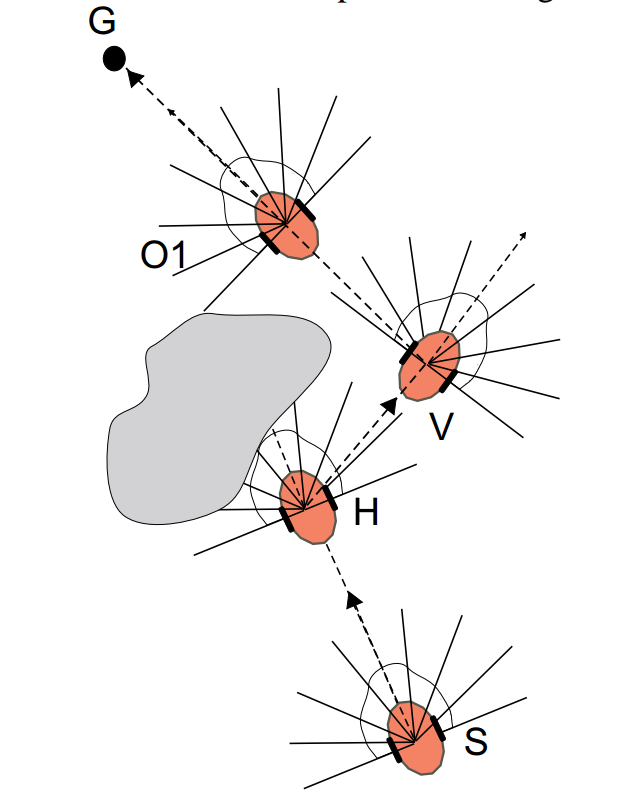
\includegraphics[width=0.45\textwidth]{figures/rebound.png}}
	\hspace{8pt}
	\caption{Phương pháp bong bóng phản ứng động}
	\label{fig:bubbleRebound}
\end{figure}

Một phương pháp cải tiến được đề xuất trong \cite{Susnea2010}. Tác giả đã cải tiến hình dạng của bong bóng, không phải là hình dạng cố định như trong \cite{Quinlan1993} mà hình dạng và kích thước được điều chỉnh liên tục dựa vào tốc độ di chuyển của robot. Khi các cảm biến phát hiện vật cản nằm trong giới hạn của bong bóng phản ứng, một thuật toán được dùng để xác định hướng của vật cản so với hướng di chuyển của robot \figurename{\ref{fig:bb-computeAngle}}. Một quá trình di chuyển của robot sử dụng phương pháp này được minh họa tại \figurename{\ref{fig:bb-reboudProcess}}.

Cũng theo tác giả \cite{Susnea2010}, phương pháp này có ưu điểm là có thể triển khai trên các thiết bị giá thành thấp, chi phí tính toán thấp nhưng có thể hoạt động theo thời gian thực. Tuy nhiên, nó cũng có một số điểm hạn chế như quá trình di chuyển chưa mượt, robot khó xử lý khi gặp nhiều vật cản đồng thời \dots

\section{Nội dung nghiên cứu}

% Chốt lại nội dung nghiên cứu gồm 2 nội dung:
% - Điều khiển robot ứng dụng SLAM trên nền tảng hệ điều hành ROS
% - Sử dụng Multi-sensor để tăng cường phát hiện và tránh vật cản cho robot
% - Trình bày vắn tắt nội dung của các chương.

Với mong muốn tiếp cận với công nghệ thế giới trong lĩnh vực robot tự hành, xe tự lái, luận văn này thực hiện 2 nhiệm vụ chính:
\begin{itemize}
  \item Cấu hình robot ứng dụng SLAM trên nền tảng hệ điều hành ROS
  \item Tăng cường phát hiện và tránh vật cản cho robot bằng đa cảm biến.
\end{itemize}

%%===========================
\chapter{Cơ sở lý thuyết}
\label{chap:1cslt}
\section{Bài toán về nhiễu trong robot tự hành}


\section{Bài toán SLAM 2D}

\section{Bài toán tạo định vị, tạo bản đồ, điều hướng và tránh vật cản}

\section{Hệ điều hành robot ROS và các ứng dụng}

% Tóm gọn nội dung giới thiệu về ROS và các ứng dụng trong khuôn khổ của luận văn này.

%% ===================
%%% Local Variables:
%%% mode: latex
%%% TeX-master: "../LuanVanThS_v1.0_main"
%%% End:
